\documentclass[12pt,letterpaper]{article}
\usepackage{graphicx,textcomp}
\usepackage{natbib}
\usepackage{setspace}
\usepackage{fullpage}
\usepackage{color}
\usepackage[reqno]{amsmath}
\usepackage{amsthm}
\usepackage{fancyvrb}
\usepackage{amssymb,enumerate}
\usepackage[all]{xy}
\usepackage{endnotes}
\usepackage{lscape}
\newtheorem{com}{Comment}
\usepackage{float}
\usepackage{hyperref}
\newtheorem{lem} {Lemma}
\newtheorem{prop}{Proposition}
\newtheorem{thm}{Theorem}
\newtheorem{defn}{Definition}
\newtheorem{cor}{Corollary}
\newtheorem{obs}{Observation}
\usepackage[compact]{titlesec}
\usepackage{dcolumn}
\usepackage{tikz}
\usetikzlibrary{arrows}
\usepackage{multirow}
\usepackage{xcolor}
\newcolumntype{.}{D{.}{.}{-1}}
\newcolumntype{d}[1]{D{.}{.}{#1}}
\definecolor{light-gray}{gray}{0.65}
\usepackage{url}
\usepackage{listings}
\usepackage{color}


\definecolor{codegreen}{rgb}{0,0.6,0}
\definecolor{codegray}{rgb}{0.5,0.5,0.5}
\definecolor{codepurple}{rgb}{0.58,0,0.82}
\definecolor{backcolour}{rgb}{0.95,0.95,0.92}

\lstdefinestyle{mystyle}{
	backgroundcolor=\color{backcolour},   
	commentstyle=\color{codegreen},
	keywordstyle=\color{magenta},
	numberstyle=\tiny\color{codegray},
	stringstyle=\color{codepurple},
	basicstyle=\footnotesize,
	breakatwhitespace=false,         
	breaklines=true,                 
	captionpos=b,                    
	keepspaces=true,                 
	numbers=left,                    
	numbersep=5pt,                  
	showspaces=false,                
	showstringspaces=false,
	showtabs=false,                  
	tabsize=2
}
\lstset{style=mystyle}
\newcommand{\Sref}[1]{Section~\ref{#1}}
\newtheorem{hyp}{Hypothesis}

\title{Applied Stats/Quant Methods 1: Problem Set 3}
\date{Due: November 11, 2024}
\author{Jamie McClenaghan}


\begin{document}
	\maketitle
	\section*{Instructions}
	\begin{itemize}
		\item Please show your work! You may lose points by simply writing in the answer. If the problem requires you to execute commands in \texttt{R}, please include the code you used to get your answers. Please also include the \texttt{.R} file that contains your code. If you are not sure if work needs to be shown for a particular problem, please ask.
	\item Your homework should be submitted electronically on GitHub.
	\item This problem set is due before 23:59 on Sunday November 11, 2024. No late assignments will be accepted.

	\end{itemize}

		\vspace{.25cm}
	
\noindent In this problem set, you will run several regressions and create an add variable plot (see the lecture slides) in \texttt{R} using the \texttt{incumbents\_subset.csv} dataset. Include all of your code.

	\vspace{15cm}
\section*{Question 1}
\vspace{.25cm}
\noindent We are interested in knowing how the difference in campaign spending between incumbent and challenger affects the incumbent's vote share. 
	\begin{enumerate}
		\item Run a regression where the outcome variable is \texttt{voteshare} and the explanatory variable is \texttt{difflog}.					\lstinputlisting[language=R, firstline=45, lastline=47]{PS3_JMcC.R} 
		
		\begin{table}[H]
\begin{center}
\begin{tabular}{l c}
\hline
 & Model 1 \\
\hline
(Intercept) & $0.58^{***}$ \\
            & $(0.00)$     \\
difflog     & $0.04^{***}$ \\
            & $(0.00)$     \\
\hline
R$^2$       & $0.37$       \\
Adj. R$^2$  & $0.37$       \\
Num. obs.   & $3193$       \\
\hline
\multicolumn{2}{l}{\scriptsize{$^{***}p<0.001$; $^{**}p<0.01$; $^{*}p<0.05$}}
\end{tabular}
\caption{Statistical models}
\label{table:coefficients}
\end{center}
\end{table}
		
		

		\item Make a scatterplot of the two variables and add the regression line. 							\lstinputlisting[language=R, firstline=49, lastline=53]{PS3_JMcC.R} 

\begin{figure}[h!]  
    \centering
    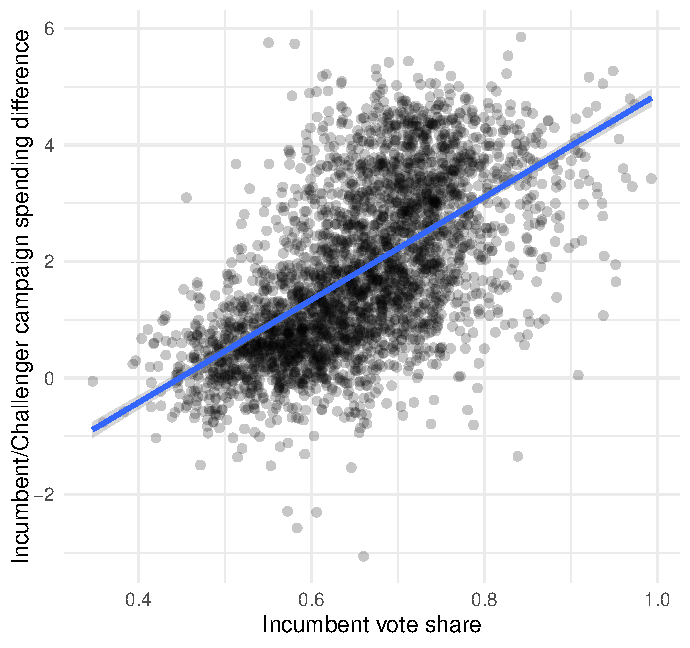
\includegraphics{Question1plot.pdf}  
\end{figure}

	\vspace{5cm}


		\item Save the residuals of the model in a separate object.							\lstinputlisting[language=R, firstline=55, lastline=56]{PS3_JMcC.R} 

		\item Write the prediction equation.
		
\begin{equation*}
			\text{voteshare} = 0.579 + 0.042 \cdot \text{difflog} + \epsilon
		\end{equation*}		
	\end{enumerate}
	
\newpage

\section*{Question 2}
\noindent We are interested in knowing how the difference between incumbent and challenger's spending and the vote share of the presidential candidate of the incumbent's party are related.	\vspace{.25cm}
	\begin{enumerate}
		\item Run a regression where the outcome variable is \texttt{presvote} and the explanatory variable is \texttt{difflog}.	
		\lstinputlisting[language=R, firstline=60, lastline=62]{PS3_JMcC.R} 
		
		\begin{table}[H]
\begin{center}
\begin{tabular}{l c}
\hline
 & Model 1 \\
\hline
(Intercept) & $0.51^{***}$ \\
            & $(0.00)$     \\
difflog     & $0.02^{***}$ \\
            & $(0.00)$     \\
\hline
R$^2$       & $0.09$       \\
Adj. R$^2$  & $0.09$       \\
Num. obs.   & $3193$       \\
\hline
\multicolumn{2}{l}{\scriptsize{$^{***}p<0.001$; $^{**}p<0.01$; $^{*}p<0.05$}}
\end{tabular}
\caption{Statistical models}
\label{table:coefficients}
\end{center}
\end{table}
	
		\item Make a scatterplot of the two variables and add the regression line. 	
		\lstinputlisting[language=R, firstline=64, lastline=68]{PS3_JMcC.R} \vspace{7cm}
		
		\begin{figure}[h!]  
    \centering
    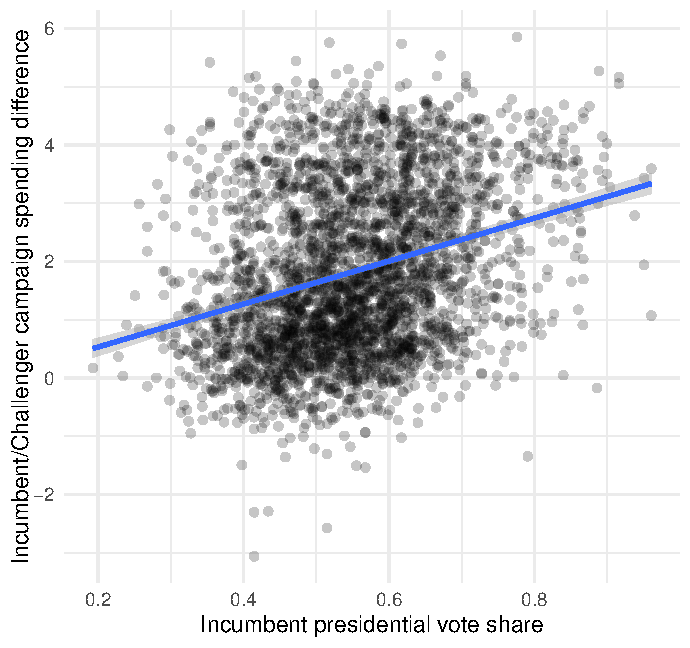
\includegraphics{Question2plot.pdf}  
\end{figure}

		
		\vspace{5cm}
		\item Save the residuals of the model in a separate object.	
		\lstinputlisting[language=R, firstline=70, lastline=71]{PS3_JMcC.R} \vspace{7cm}
		\vspace{5cm}
		\item Write the prediction equation.
		
				\begin{equation*}
			\text{presvote} = 0.508 + 0.024 \cdot \text{difflog} + \epsilon
		\end{equation*}

		
	\end{enumerate}
	
	\newpage	
\section*{Question 3}

\noindent We are interested in knowing how the vote share of the presidential candidate of the incumbent's party is associated with the incumbent's electoral success.
	\vspace{.25cm}
	\begin{enumerate}
		\item Run a regression where the outcome variable is \texttt{voteshare} and the explanatory variable is \texttt{presvote}.
				\lstinputlisting[language=R, firstline=75, lastline=77]{PS3_JMcC.R} 
				\begin{table}[H]
\begin{center}
\begin{tabular}{l c}
\hline
 & Model 1 \\
\hline
(Intercept) & $0.44^{***}$ \\
            & $(0.01)$     \\
presvote    & $0.39^{***}$ \\
            & $(0.01)$     \\
\hline
R$^2$       & $0.21$       \\
Adj. R$^2$  & $0.21$       \\
Num. obs.   & $3193$       \\
\hline
\multicolumn{2}{l}{\scriptsize{$^{***}p<0.001$; $^{**}p<0.01$; $^{*}p<0.05$}}
\end{tabular}
\caption{Statistical models}
\label{table:coefficients}
\end{center}
\end{table}
				
		\item Make a scatterplot of the two variables and add the regression line. 
				\lstinputlisting[language=R, firstline=79, lastline=83]{PS3_JMcC.R} \vspace{7cm}
				
				\begin{figure}[h!]  
    \centering
    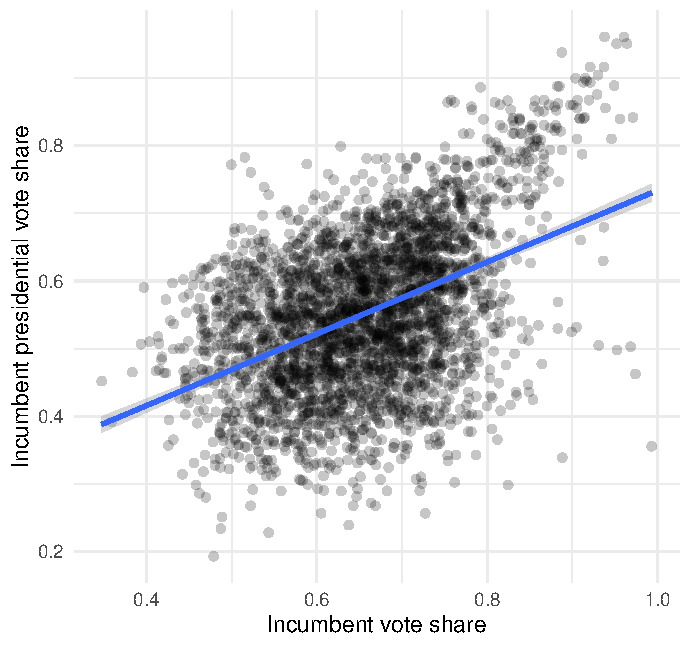
\includegraphics{Question3plot.pdf}  
\end{figure}

				
			\vspace{5cm}
		\item Write the prediction equation.
		
		\begin{equation*}
			\text{voteshare} = 0.441 + 0.388 \cdot \text{presvote} + \epsilon
		\end{equation*}
		
	\end{enumerate}
	

\newpage	
\section*{Question 4}
\noindent The residuals from part (a) tell us how much of the variation in \texttt{voteshare} is $not$ explained by the difference in spending between incumbent and challenger. The residuals in part (b) tell us how much of the variation in \texttt{presvote} is $not$ explained by the difference in spending between incumbent and challenger in the district.
	\begin{enumerate}
		\item Run a regression where the outcome variable is the residuals from Question 1 and the explanatory variable is the residuals from Question 2.	
		
						\lstinputlisting[language=R, firstline=90, lastline=94]{PS3_JMcC.R} 
						
						\begin{table}[H]
\begin{center}
\begin{tabular}{l c}
\hline
 & Model 1 \\
\hline
(Intercept)     & $-0.00$      \\
                & $(0.00)$     \\
Model2Residuals & $0.26^{***}$ \\
                & $(0.01)$     \\
\hline
R$^2$           & $0.13$       \\
Adj. R$^2$      & $0.13$       \\
Num. obs.       & $3193$       \\
\hline
\multicolumn{2}{l}{\scriptsize{$^{***}p<0.001$; $^{**}p<0.01$; $^{*}p<0.05$}}
\end{tabular}
\caption{Statistical models}
\label{table:coefficients}
\end{center}
\end{table}

		\item Make a scatterplot of the two residuals and add the regression line. 	\
		
						\lstinputlisting[language=R, firstline=96, lastline=100]{PS3_JMcC.R} \vspace{7cm}
						
						\begin{figure}[h!]  
    \centering
    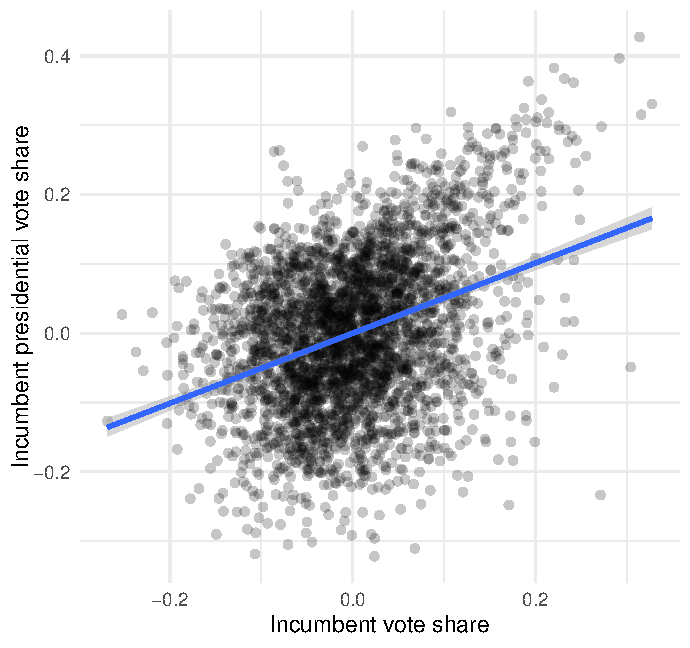
\includegraphics{Question5plot.pdf}  
\end{figure}

		
		\item Write the prediction equation.
		
		\begin{equation*}
			\text{Model1Residuals} = 0.257 \cdot \text{Model2Residuals} + \epsilon
		\end{equation*}

	\end{enumerate}
	
	\newpage	

\section*{Question 5}
\noindent What if the incumbent's vote share is affected by both the president's popularity and the difference in spending between incumbent and challenger? 
	\begin{enumerate}
		\item Run a regression where the outcome variable is the incumbent's \texttt{voteshare} and the explanatory variables are \texttt{difflog} and \texttt{presvote}.	
		
								\lstinputlisting[language=R, firstline=104, lastline=105]{PS3_JMcC.R} 
		
		\begin{table}[H]
\begin{center}
\begin{tabular}{l c}
\hline
 & Model 1 \\
\hline
(Intercept) & $0.45^{***}$ \\
            & $(0.01)$     \\
difflog     & $0.04^{***}$ \\
            & $(0.00)$     \\
presvote    & $0.26^{***}$ \\
            & $(0.01)$     \\
\hline
R$^2$       & $0.45$       \\
Adj. R$^2$  & $0.45$       \\
Num. obs.   & $3193$       \\
\hline
\multicolumn{2}{l}{\scriptsize{$^{***}p<0.001$; $^{**}p<0.01$; $^{*}p<0.05$}}
\end{tabular}
\caption{Statistical models}
\label{table:coefficients}
\end{center}
\end{table}

		\item Write the prediction equation.			
		\begin{equation*}
			\text{voteshare} = 0.449 + 0.036 \cdot \text{difflog} + 0.257 \cdot \text{presvote} + \epsilon
		\end{equation*}
				
		\item What is it in this output that is identical to the output in Question 4? Why do you think this is the case?
		
		
		The regression between the residuals from Question 1 and Question 2 in Table 4 shows a positive and significant coefficient (0.257) for Model2Residuals, this would suggest to us that the unexplained variation in \texttt{voteshare} is positively correlated with unexplained variation in \texttt{presvote}.  
		
		The coefficient for \texttt{presvote} is the same in in Table 5 and this would suggest that the unexplained variation in \texttt{voteshare} and \texttt{presvote} are closely related, and that the \texttt{difflog} control for campaign spending differences did not affect this relationship.
	
		Overall, the coefficients identical nature suggests that the unexplained variation in voteshare and presvote is highly correlated, and the influence of presvote on voteshare remains the same even after we account for the campaign spending differences.
		
	\end{enumerate}




\end{document}
